\subsection{Misura della capacità di pilotaggio}

\begin{wrapfigure}[16]{l}{0.55\textwidth}
  \begin{center}
    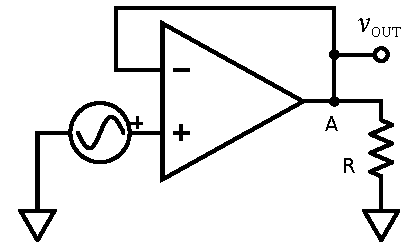
\includegraphics[width=0.26\textwidth]{../E03/latex/max_current.pdf}
  \end{center}
  \caption{Schema del circuito utilizzato per misurare la corrente massima. La resistenza utilizzata è $R=98.47\pm0.01$\si{\ohm}; il generatore fornisce un'onda triangolare di $f=1$ \si{\kilo\hertz} e $5 V_{pp}$.}
  \label{cir3:max_current}
\end{wrapfigure}

L'amplificatore operazionale ha un valore massimo di corrente erogabile in uscita. Dunque, se montiamo un circuito di feedback come in Figura \ref{cir3:max_current}, la tensione massima ai capi di $R$ sarà fissata dalla corrente massima e dal valore della resistenza stessa, da questa relazione:
\begin{equation*}
	I_{max} = \frac{V_{clip}}{R}
\end{equation*}
dove $V_{clip}$ è la tensione in cui il segnale in uscita risulta tagliato rispetto a quello in ingresso (fenomeno del \textit{clipping}).

Per misurare $I_{max}$ abbiamo dunque sfruttato questo fatto, ponendo una resistenza di carico fra l'uscita dell'operazionale e terra\footnote{Si noti che, data l'alta impedenza in ingresso dell'oscilloscopio (\SI{1}{\mega\ohm}), non era possibile misurare la corrente massima con questo strumento (attesa, come da specifiche del costruttore, sui \SI{15}{\milli\ampere}): sarebbe servita una tensione di \SI{15000}{\volt}!}, con l'oscilloscopio ai capi di tale resistenza per la misura di tensione (circuito in Figura \ref{cir3:max_current}).

\begin{figure}[ht]
 \centering
   {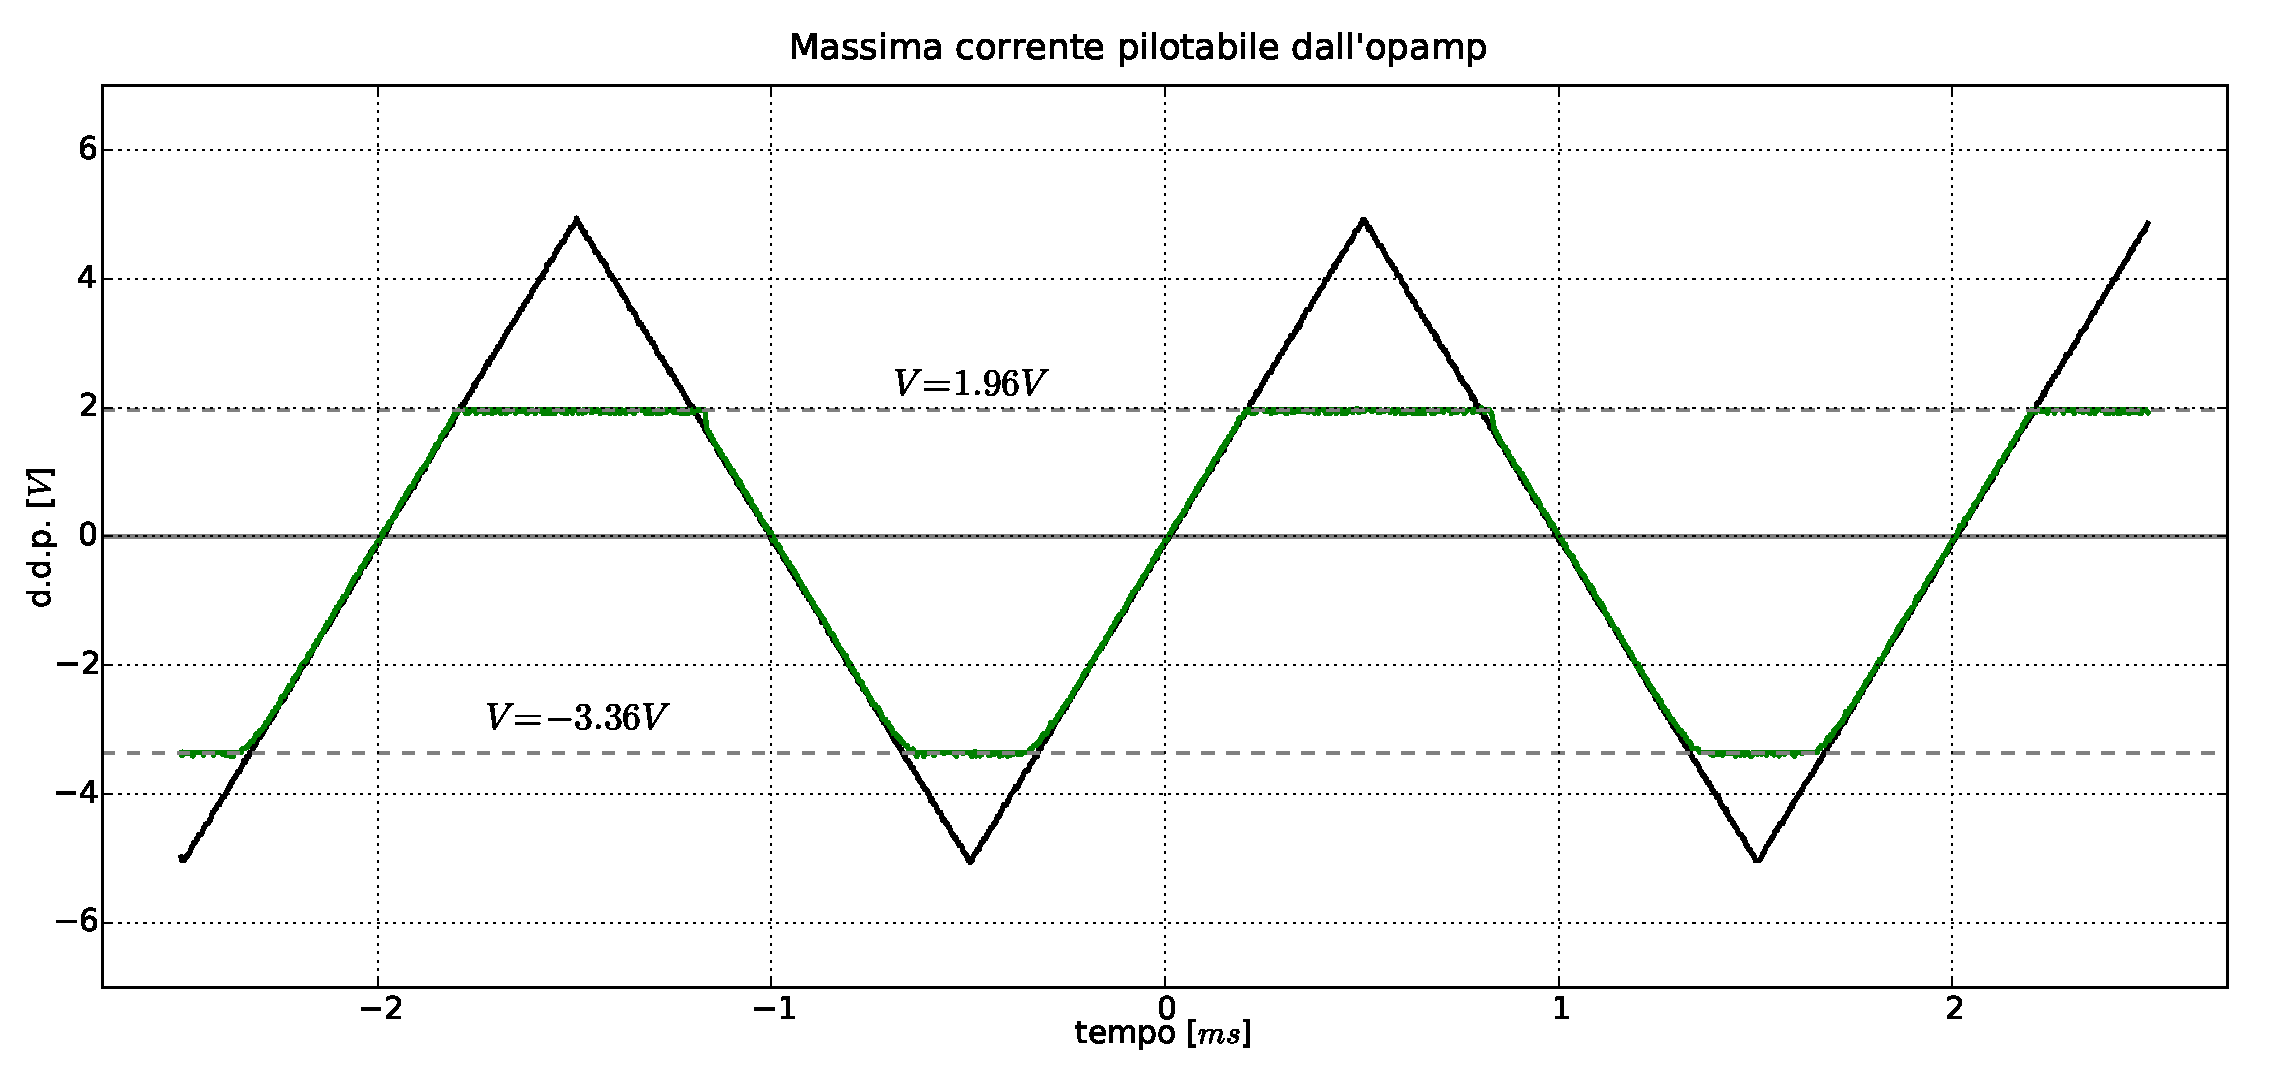
\includegraphics[width=\textwidth]{../E03/latex/clip.pdf}}
 \caption{Grafico della tensione in uscita (verde) ed in entrata (nero) in funzione del tempo. Si nota subito che il clip a tensioni negative avviene a tensioni in modulo maggiori.}
 \label{gr3:clip}
\end{figure}

Bisogna però considerare che la corrente, ponendo il segnale in entrata in alternata, risulta oscillare fra valori negativi e positivi (corrente rispettivamente entrante o uscente dal punto A). Inoltre, tali valori sono differenti (si nota dal grafico in Figura \ref{gr3:clip} l'asimmetria della tensione di clip). Infatti, se consideriamo $V^+ = (1.92 \pm 0.01)$ \si{\volt} la tensione di clip positiva e $V^- = (3.45 \pm 0.01)$ \si{\volt} quella negativa, otteniamo

$$I_{V^+} = \frac{V^+}{R} = (19.5 \pm 0.1) \si{\milli\volt}  \qquad I_{V^-} = \frac{V^-}{R} = (35.2 \pm 0.2) \si{\milli\volt}$$

Entrambi i valori sono compatibili quelli del costruttore (valori di corrente fino a $\pm 40$ \si{\milli\volt}). Questo fatto può essere spiegato considerando che la circuiteria interna dell'opamp è composta, come già più volte ribadito, da diversi transistor che solo idealmente possono essere tutti delle medesime ed identiche caratteristiche: ciò comporta una asimmetria che può spiegare il fenomeno.
